% TESTS
% implementación en MTSA, explicación mini de la herramienta
% hicimos tests, medio TDD
%-------------------------------------------------------
\begin{frame}{Herramienta MTSA}
    \begin{itemize}
    	\item El LaFHIS, donde hicimos esta tesis, trabaja hace años en MTSA, una herramienta propia para resolver problemas de control con LTS.
    	\item Implementamos el algoritmo en java, agregándolo a las capacidades de MTSA. Esto permitió ejecutar los tests y el benchmark de la próxima sección.
    \end{itemize}
\end{frame}
%-------------------------------------------------------
\begin{frame}{Test Driven Development}
	\begin{itemize}
		\item Para ganar seguridad en nuestro código, y encontrar errores, fuimos armando una batería de tests.
		\item Con cada error encontrado en la implementación o la especificación del algoritmo, armábamos un nuevo test que detectara ese error, y luego lo arreglábamos.
		\item Quedaron 49 tests pequeños diseñados a mano para correr rápido y presentar las condiciones más problemáticas para nuestro algoritmo.
		\item Ésta batería de tests fue añadida a las utilizadas por la herramienta como tests de regresión para alertar problemas por futuros cambios en el código.
	\end{itemize}
\end{frame}
%-------------------------------------------------------
\begin{frame}{Ejemplo de MTSA en uso}
	\begin{figure}
		\hspace{-2cm}
		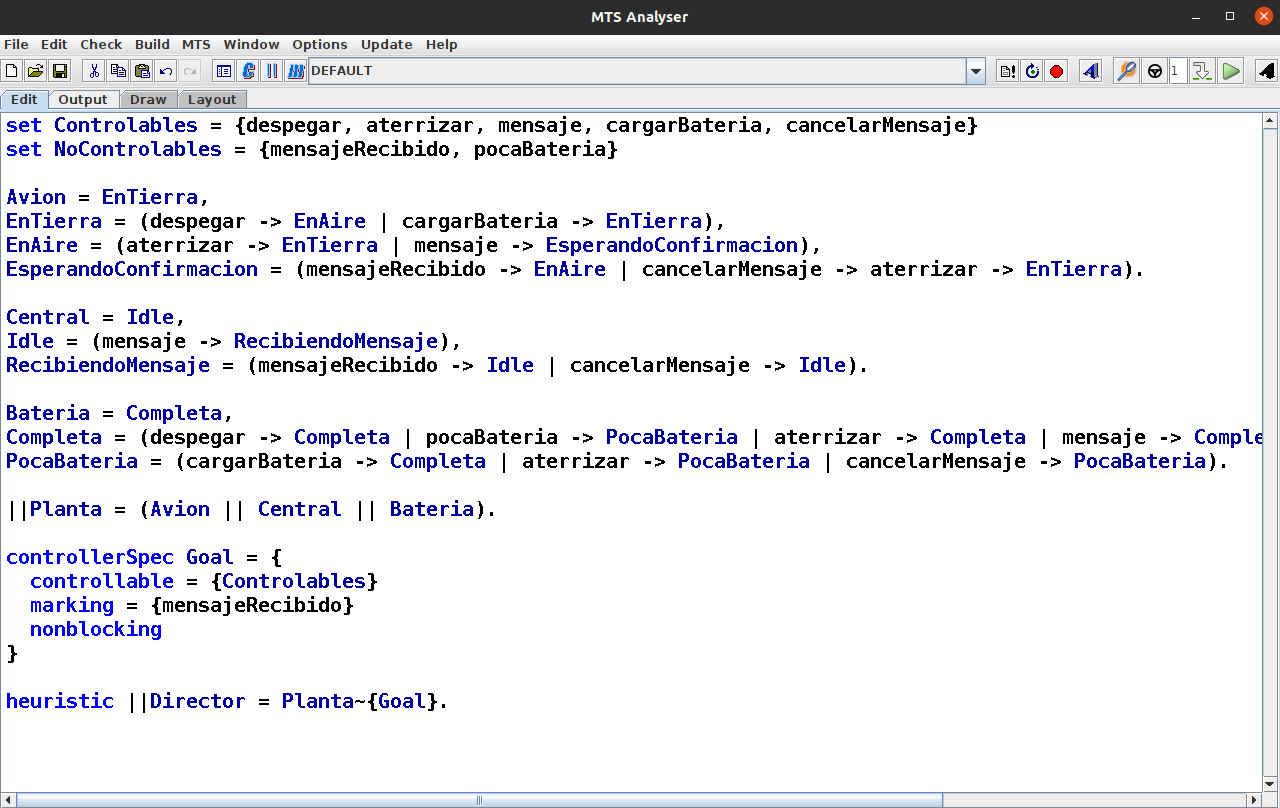
\includegraphics[width=\textwidth]{figures/HPWindow-ej.png}
	\end{figure}
	\pause
	\begin{picture}(0,0)
		\put(70,-10){
			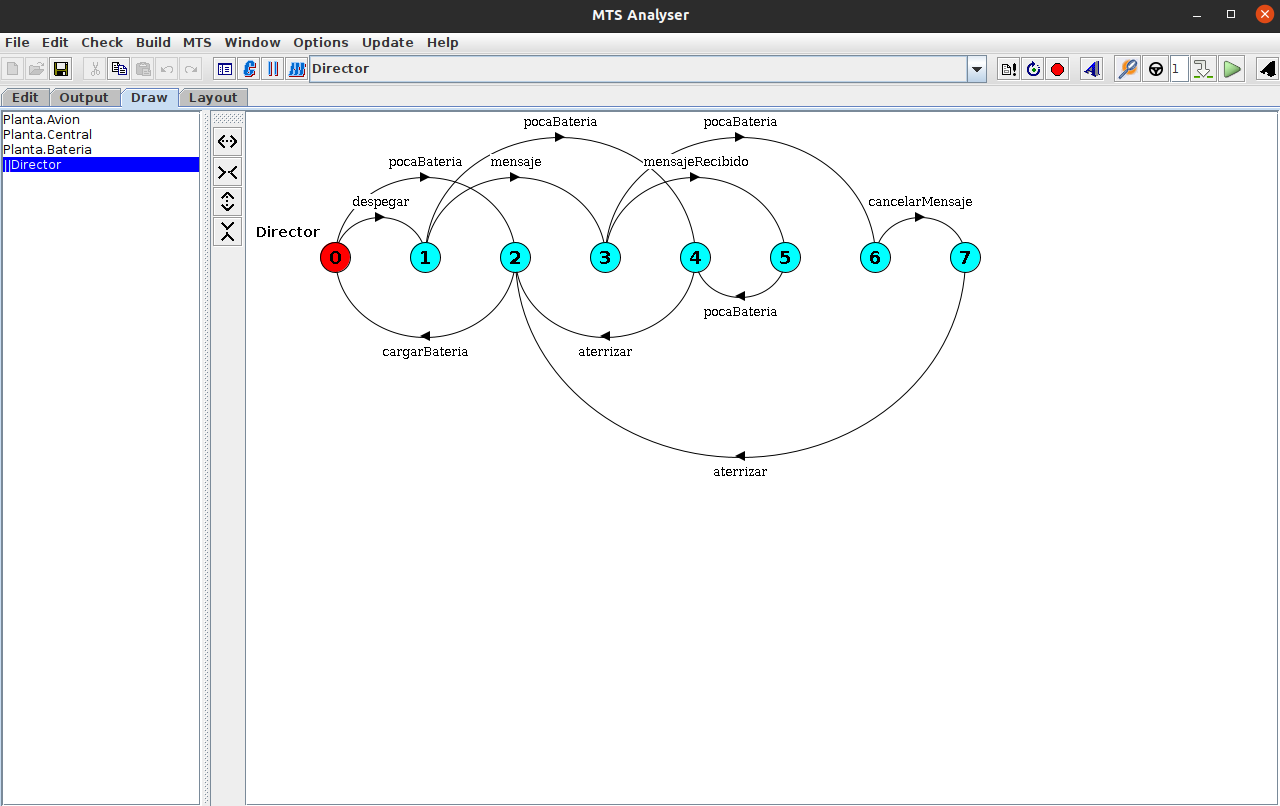
\includegraphics[width=\textwidth]{figures/controller-drawing-ej.png}
		}
	\end{picture}
\end{frame}
%-------------------------------------------------------
\begin{frame}{Animando controladores}
	Video de controlador animado?
\end{frame}
%-------------------------------------------------------
